\documentclass{article}
\usepackage[utf8]{inputenc}
\usepackage{geometry}
\usepackage{pdfpages}
\usepackage{filecontents}
\graphicspath{{images/}}
\geometry{
	a4paper,
	total={170mm,257mm},
	left=20mm,
	top=20mm,
}
\usepackage{graphicx}
\usepackage{titling}
\usepackage[american,RPvoltages]{circuiTikz}
\usepackage{tikz, tikz-cd}
\usepackage{pgfplots}
\usepackage{siunitx}
\usepackage{float}
\usepackage{enumitem}
\usepackage{amsmath,amsfonts,stmaryrd,amssymb} % Math packages
\usepackage{schemabloc}
\usepackage{tcolorbox}
\title{Diseño con OpAmp}
\author{Rodrigo}
\date{Agosto 2024}

\usepackage{fancyhdr}
\fancypagestyle{plain}{%  the preset of fancyhdr 
	\fancyhf{} % clear all header and footer fields
	\fancyfoot[L]{\thedate}
	\fancyhead[L]{Diseño con OpAmp}
	\fancyhead[R]{\theauthor}
}
\makeatletter
\def\@maketitle{%
	\newpage
	\null
	\vskip 1em%
	\begin{center}%
		\let \footnote \thanks
		{\LARGE \@title \par}%
		\vskip 1em%
		%{\large \@date}%
	\end{center}%
	\par
	\vskip 1em}
\makeatother

\usepackage{lipsum}  
\usepackage{cmbright}

%---------------------------------------------------
\tikzset{flipflop myRS/.style={flipflop,
		 flipflop def={t1=R, t3=S, t6=Q, t4={\ctikztextnot{Q}}, tu={\ctikztextnot{RST}}, nu=1, n4=1 }}
	}
	
\tikzset{flipflop myFFRS/.style={flipflop,
		flipflop def={t1=R, t3=S, t6=Q, t4={\ctikztextnot{Q}}, n4=1 }}
}
%---------------------------------------------------

\makeatletter
\newcommand*{\underarrow}{\def\@underarrow{\relax}\@ifstar{\@@underarrow}{\def\@underarrow{\hidewidth}\@@underarrow}}
\newcommand*{\@@underarrow}[2][]{\underset{\@underarrow\substack{\uparrow\if\relax\detokenize{#1}\relax\else\\#1\fi}\@underarrow}{#2}}

\newcommand*{\overarrow}{\def\@overarrow{\relax}\@ifstar{\@@overarrow}{\def\@overarrow{\hidewidth}\@@overarrow}}
\newcommand*{\@@overarrow}[2][]{\overset{\@overarrow\substack{\if\relax\detokenize{#1}\relax\else#1\\\fi\downarrow}\@overarrow}{#2}}
\makeatother

\begin{document}
	
\maketitle
	
\noindent\begin{tabular}{@{}ll}
Author & \theauthor\\
\end{tabular}
	
\section*{Problema}
Una termocupla de cromo-constantán tiene las características que se muestra en la siguiente figura (curva E). Diseñe una interface que produzca una salida de $\qty{-5}{\volt}$ a $\qty{+5}{\volt}$, donde $\qty{-5}{\volt}$ hace referencia a 0°C y $\qty{+5}{\volt}$ a $\qty{1000}{\degreeCelsius}$. El transductor puede ser modelado como una fuente de voltaje en serie con un resistor de $\qty{15}{\ohm}$. \\


\noindent De la gráfica podemos observar que la recta perteneciente a $E$ cruza exactamente por el punto $(\qty{400}{\degreeCelsius},\qty{30}{\milli \volt})$, con esto obtenemos dos pares de coordenadas, a saber:

\begin{align}
	P_1\underbrace{(0,0)}_\text{$x_1$, $y_1$} \qquad P_2\underbrace{(400,30)}_\text{$x_2$, $y_2$}
\end{align}

\noindent Con el par de coordenadas mostrado en (1) podemos construir una ecuación lineal de la forma $y = \pm mx \pm b $, donde los parámetros $m$ y $b$ representan la \textit{pendiente} y la \textit{ordenada} al origen, respectivamente. Para la construcción de la recta utilizamos la \textbf{Ecuación de la recta que pasa por dos puntos}:

\subsection*{Ecuación de la recta que pasa por dos puntos}
Dados los puntos $P_1(x_1, y_1)$ y $P_2(x_2, y_2)$ de la recta, su ecuación es:

\begin{align}
	y - y_1 = \frac{y_2 - y_1}{x_2 - x_1}(x - x_1)
\end{align}

\begin{figure}[H]
	\centering	
	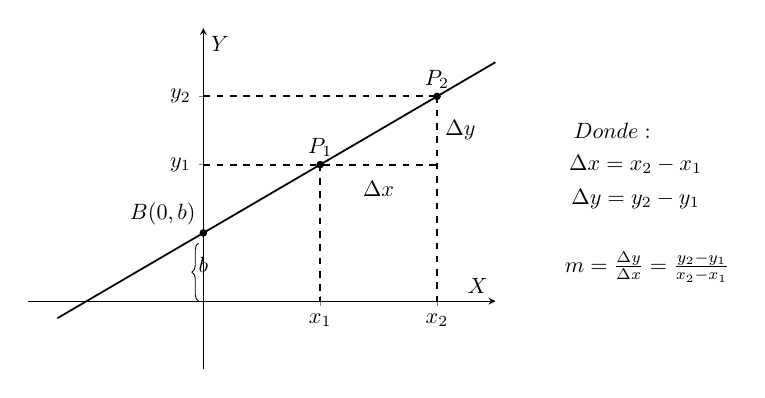
\begin{tikzpicture}[scale=0.8, transform shape]
		\pgfplotsset{width=9cm,height=7cm,compat=1.18}
		\begin{axis}[xshift=6cm,
			yshift=2cm,
			clip=false,
			axis y line=left,
			axis x line=middle,
			xlabel=$X$,
			ylabel=$Y$, 
			axis y line= center,
			xmin=-3,xmax=5,
			ymin=-2,ymax=8,
			xtick={2, 4},
			ytick={4, 6},
			xticklabels={$x_1$,$x_2$},
			yticklabels={$y_1$,$y_2$},
			]
			\addplot[smooth, black,thick, mark=none, domain=-2.5:5, samples=200] {x + 2};
			\addplot[color = black, dashed, thick] coordinates {(2,4) (2,0)}; %vertical1
			\addplot[color = black, dashed, thick] coordinates {(4,6) (4,0)}; %vertical2
			\addplot[color = black, dashed, thick] coordinates {(0,4) (4,4)}; %horizontal1
			\addplot[color = black, dashed, thick] coordinates {(0,6) (4,6)}; %horizontal2
			\draw[fill=black](2,4) circle (1.5pt) node [above] {$P_1$};
			\draw[fill=black](4,6) circle (1.5pt) node [above] {$P_2$};
			\draw[fill=black](0,2) circle (1.5pt) node [above left] {$B(0,b)$};
			\node[] at (axis cs:3,3.3){$\Delta x$};
			\node[] at (axis cs:4.4,5){$\Delta y$};
			\draw [decorate,decoration={brace,amplitude=3pt,raise=0.5ex}] (0,0) -- (0,1.7) node[left=4mm, below=1mm]{$b$};
			\node[] at (axis cs:7,5){$Donde:$};
			\node[] at (axis cs:7.4,4){$\Delta x = x_2 - x_1 $};
			\node[] at (axis cs:7.4,3){$\Delta y = y_2 - y_1 $};
			\node[] at (axis cs:7.6,1){$m = \frac{\Delta y}{\Delta x} = \frac{y_2 - y_1}{x_2 - x_1} $};
		\end{axis}
	\end{tikzpicture}
	\caption{Línea Recta}	
	\label{fig:figura1}
\end{figure}



\noindent Al sustituir los valores dados en (1) en la ecuación (2) obtenemos:
\begin{align}
	y - 0 &= \frac{30 - 0}{400 - 0}(x - 0) \nonumber \\
	y &= \frac{30}{400}x \nonumber
\end{align}

o bien

\begin{align}
	y = \frac{\overarrow[mV]{3}}{40}x
\end{align}

\begin{figure}[H]
	\centering	
	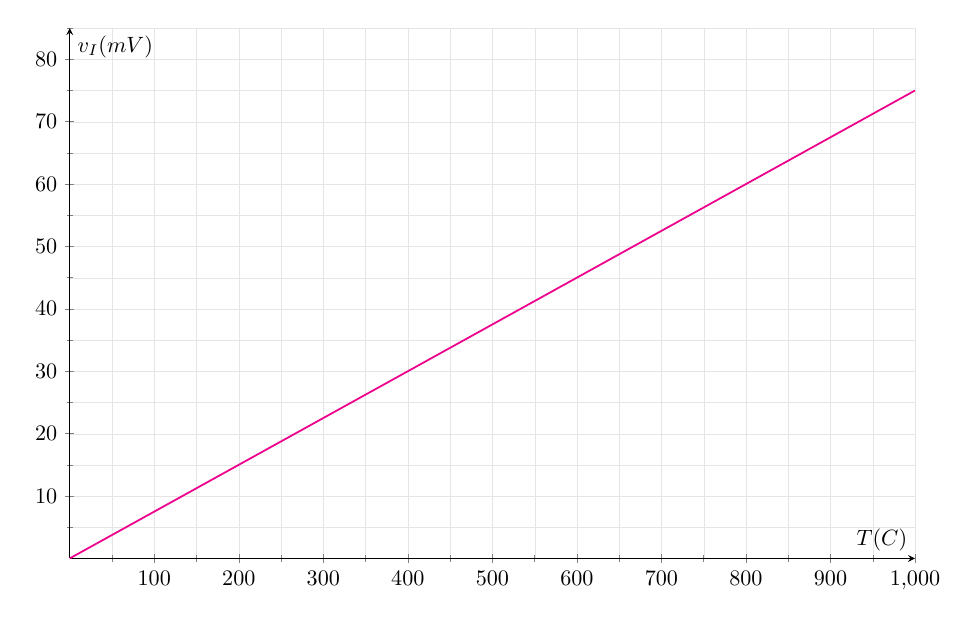
\begin{tikzpicture}[scale=0.8, transform shape]
		  \pgfplotsset{width=15cm,height=10cm,compat=1.18}
		  \begin{axis}[xshift=6cm,
		  	yshift=2cm,
		  	clip=false,
		  	axis y line=left,
		  	axis x line=middle,
		  	grid style={line width=.1pt, draw=gray!20},
		  	grid=both,
		  	minor tick num=1,
		  	xlabel=$\quad T (°C)$,
		  	ylabel=$v_I (mV)$, 
		  	axis y line= center,
		  	xmin=0,xmax=1000,
		  	ymin=0,ymax=85,
		  	%xtick={0, 10, 20, 30, 40, 50, 60, },
		  	%ytick={1},
		  	%xticklabels={$$},
		  	%yticklabels={$V_{CC}$},
		  	]
		    \addplot[smooth, magenta,thick, mark=none, domain=0:1000, samples=200] {(3/40)*x};
		  \end{axis}
	\end{tikzpicture}
	\caption{Gradiente de temperatura para una termocupla de cromo-constantán}	
	\label{fig:figura7}
\end{figure}

Con la ecuación dada en (3) podemos fácilmente predecir el voltaje a cualquier temperatura dada, lo reescribiremos empleando las unidades correspondientes:

\begin{align}
	V_o [mV] = \frac{3}{40}T [^\circ C]
\end{align}

\noindent Ahora, el objetivo del diseño es diseñar una interface que produzca una salida en el rango de $-5 \leq V_o \leq +5$ para una temperatura en el rango de $0 \leq T \leq 1000$. Utilizamos (4) para conocer los valores del sensor dadas las temperaturas $T_1 = \qty{0}{\degreeCelsius}$ y $T_2 = \qty{1000}{\degreeCelsius}$

\begin{align}
	V_{sensor_1} &= \frac{3}{40}(0) = \qty{0}{\volt} \\
	V_{sensor_2} &= \frac{3}{40}(1000) = \qty{75}{\milli \volt}
\end{align}

\noindent Ya tenemos los dos valores de entrada y los dos valores de salida por lo que podemos armar nuevamente un segundo par de coordenadas como se muestra a continuación. 

\begin{align}
	P_1\underbrace{(V_{sensor_1},V_{out_1})}_\text{$x_1$, $y_1$} &\qquad P_2\underbrace{(V_{sensor_2}, V_{out_2})}_\text{$x_2$, $y_2$} \nonumber \\
	P_1 (0, -5) &\qquad P_2 (0.075, 5)
\end{align}

\noindent Es decir, cuando el voltaje de entrada $V_{sensor_1} = 0$ el voltaje de salida será de $V_{out_1} = \qty{-5}{\volt}$ y cuando el voltaje de entrada $V_{sensor_2} = \qty{75}{\milli \volt}$ el voltaje de salida será de $V_{out_1} = \qty{5}{\volt}$

\noindent Con el par de coordenadas dadas en (7) utilizamos nuevamente la ecuación (2)

\begin{align}
	y - (-5) &= \frac{5 - (-5)}{0.075 - 0}(x - 0) \nonumber \\
	y + 5&= \frac{10}{0.075}x \nonumber \\
	y &=  \frac{400}{3}x - 5 \nonumber
\end{align}

Reescribiendo la ecuación anterior con las unidades apropiades obtenemos

\begin{align}
	V_{out} =  \left( \frac{400}{3} \right)V_{sensor} - 5
\end{align}

La ecuación en (8) nos sugeriría un diseño como el que se muestra en el diagrama de bloques de la figura 3, el cual es de hecho, el de un amplificador sumador. Para este diseño, emplearemos un amplificador sumador inversor como el que se muestra en la figura 4.
\begin{figure}[H]
	\centering	
	\begin{tikzpicture}[scale=0.8]
		\ctikzset{bipoles/thickness=4}
		\ctikzset{monopoles/vcc/arrow={Stealth[width=6pt,length=9pt]}}
		\ctikzset{monopoles/vee/arrow={Stealth[width=6pt,length=9pt]}}
		\node[mixer, fill=cyan!10](A) at (0,0){};
		\draw (A.center) node[above]{$+$};
		\draw (A.center) node[below]{$+$};
		\draw (A.n) to[short] ++(0,1) to[short] ++(-2,0) coordinate (p1);
		\draw (A.s) to[short] ++(0,-1) to[short] ++(-2,0) coordinate (p2);
		\node[twoportshape, t=$K_1$, anchor=e, fill=cyan!10](B) at (p1){};
		\node[twoportshape, t=$K_2$, anchor=e, fill=cyan!10](C) at (p2){};
		\draw[Stealth-](C.w) -- ++(-1,0) node[above]{$v_2$};
		\draw[Stealth-](A.s) -- ++(0,-1);
		\draw[Stealth-](A.n) -- ++(0,1);
		\draw[Stealth-](B.w) -- ++(-1,0) node[above]{$v_1$};
		\draw[-Stealth](A.e) -- ++(1,0) node[right]{$v_o$};
	\end{tikzpicture}
	\caption{Diagrama de bloques de un amplificador sumador}	
	\label{fig:figura5}
\end{figure}

\noindent La ecuación de salida de un amplificador no inversor está dada por

\begin{align}
	v_o = -\frac{R_F}{R_1}v_1 - \frac{R_F}{R_2}v_2
\end{align}

\noindent Donde

\begin{align}
	K_1 = -\frac{R_F}{R_1} \qquad K_2 = -\frac{R_F}{R_2}
\end{align}
\begin{figure}[H]
	\centering
	\begin{tikzpicture}[scale=0.8]
		\ctikzset{bipoles/thickness=4}
		\ctikzset{monopoles/vcc/arrow={Stealth[width=6pt,length=9pt]}}
		\ctikzset{monopoles/vee/arrow={Stealth[width=6pt,length=9pt]}}
		\draw (0,0) node[op amp, anchor=+](OA){};
		\draw (OA.-) to[short] ++(-1,0)
		      to[short, -*] ++(0,2) coordinate (p1);
		\draw (p1) to[R, l=$R_F$]  (p1 -| OA.out) to[short, -*] (OA.out);
		\draw (OA.out) to[short, -o] ++(0.5,0) node[right]{$v_O$};
		\draw (p1) to[short] ++(-1,0) coordinate (p2);
		\draw(p2) to[R, -o, l_=$R_1$] ++ (-3,0) node[left]{$v_1$};
		\draw (p2) to[short, *-] ++(0,-2)
		      to[R, -o, l_=$R_2$] ++ (-3,0) node[left]{$v_2$};
		\draw (OA.+) to[short] ++(-1,0) to[short] ++(0,-1) node[ground]{};
		%\draw(OA.up) to[short] ++(0,0.4) node[vcc](VCC){$+V_{CC}$};
		%\draw(OA.down) to[short] ++(0,-0.4) node[vee](VEE){$-V_{EE}$};
	\end{tikzpicture}
	\caption{Amplificador sumador inversor}	
	\label{fig:figura6}
\end{figure}

\noindent En la ecuación (9) observamos que el voltaje de salida es negativa en ambos operandos, sin embargo, la ecuación (8) sugiere que el primer término debe ser positivo. La forma de volver positivo el primer término en (9) es inviertiendo dicha señal, esto se logra conectando un amplificador inversor en la entrada de $v_1$ en el diagrama de la figura 3, esta modificación se muestra en el diagrama de la figura 5.

\begin{figure}[H]
	\centering	
	\begin{tikzpicture}[scale=0.8]
		\ctikzset{bipoles/thickness=4}
		\ctikzset{monopoles/vcc/arrow={Stealth[width=6pt,length=9pt]}}
		\ctikzset{monopoles/vee/arrow={Stealth[width=6pt,length=9pt]}}
		\node[mixer, fill=cyan!10](A) at (0,0){};
		\draw (A.center) node[above]{$+$};
		\draw (A.center) node[below]{$+$};
		\draw (A.n) to[short] ++(0,1) to[short] ++(-2,0) coordinate (p1);
		\draw (A.s) to[short] ++(0,-1) to[short] ++(-3.1,0) coordinate (p2);
		\node[twoportshape, t=$-1$, anchor=e, fill=cyan!10](B) at (p1){};
		\node[twoportshape, t=$K_2$, anchor=e, fill=cyan!10](C) at (p2){};
		\draw[Stealth-](C.w) -- ++(-2.15,0) node[left]{$v_2$};
		\draw[Stealth-](A.s) -- ++(0,-1);
		\draw[Stealth-](A.n) -- ++(0,1);
		\draw[Stealth-](B.w) -- ++(-1,0) coordinate(p3);
		\node[twoportshape, anchor=e, fill=cyan!10, t=$K_1$](D) at (p3){};
		\draw[Stealth-](D.w) -- ++(-1,0) node[left]{$v_1$};
		\draw[-Stealth](A.e) -- ++(1,0) node[right]{$v_o$};
	\end{tikzpicture}
	\caption{Diagrama de bloques }	
	\label{fig:figura8}
\end{figure}

La ecuación de salida está dada ahora por:
\begin{align}
	v_o = \frac{R_F}{R_1}v_1 - \frac{R_F}{R_2}v_2
\end{align}

\noindent Comparemos ahora la ecuación (11) con la ecuación (8)
\begin{align}
	v_o &= \underbrace{\frac{R_F}{R_1}}_\text{m}\underbrace{v_1}_\textbf{x} - \underbrace{\frac{R_F}{R_2}v_2}_\text{b} \\
	V_{o} &=  \underbrace{\left( \frac{400}{3} \right)}_\text{m}\underbrace{V_{sensor}}_\text{x}  - \underbrace{5}_\text{b}
\end{align}

\noindent Por simplicidad, la ganancia del amplificador inversor será de $1$. Ahora, al igualar términos obtenemos
\begin{align}
	\frac{R_F}{R_1} =\frac{400}{3} \nonumber
\end{align}

\noindent O

\begin{align}
	R_1 = \frac{3}{400}R_F \nonumber
\end{align}

\noindent Si establecemos $R_F = \qty{100}{\kilo \ohm}$, entonces $R_1 = \qty{750}{\ohm}$. Ya tenemos la ganancia $K_1$ (figura 5), nos faltaría la ganancia $K_2$ que de acuerdo a la ecuación (13), ésta sería de $5$. La ecuación (12) nos indica que debemos tener una señal de entrada llamada $v_2$. Podemos aprovechar la tensión de alimentación positiva que conectaremos al OpAmp para poder obtener esa señal de voltaje $v_2$. Supongamos que a nuestro OmAmp lo alimentamos con una fuente de $V_{{CC}} = \qty{15}{\volt}$ y $V_{{EE}} = \qty{-15}{\volt}$. Una opción sería bajar el voltaje de $\qty{15}{\volt}$ a $\qty{1}{\volt}$ a través de un simple divisor de tensión con dos resistores, ese voltaje de $\qty{1}{\volt}$ sería la entrada $v_2$ y al establecer la ganancia $\frac{R_F}{R_2} = 5$ cumpliríamos con la condición de $\frac{R_F}{R_2}v_2 = 5$, donde $v_2 = \qty{1}{\volt}$\\

\noindent Sólo nos queda establecer la relación:

\begin{align}
	\frac{R_F}{R_2} = 5\nonumber \\
	R_F = 5R_2 \nonumber \\
	R_2 = \frac{R_F}{5} \nonumber
\end{align}

\noindent Ya que establecimos $R_F = \qty{100}{\kilo \ohm}$, entonces $R_1 = \qty{20}{\kilo \ohm}$. Diseñemos ahora la red divisora de voltaje para obtener un voltaje de $\qty{1}{\volt}$ a partir del voltaje de alimentación $V_{CC} = \qty{15}{\volt}$. Sea el siguiente circuito:

\begin{figure}[H]
	\centering	
	\begin{tikzpicture}[scale=0.8]
		\ctikzset{bipoles/thickness=4}
		\ctikzset{monopoles/vcc/arrow={Stealth[width=6pt,length=9pt]}}
		\ctikzset{monopoles/vee/arrow={Stealth[width=6pt,length=9pt]}}
		\draw (0,0) node[vcc](VCC){$+V_{CC}$} to[R, l=$R_a$] ++(0,-3) coordinate (p1)
		      to[short, -o] ++(2,0) node[right]{$V_a = \qty{1}{\volt}$};
		\draw (p1) to[R, *-, l=$R_b$] ++(0,-3) node[ground]{};
	\end{tikzpicture}
	\caption{Red divisora de voltaje }	
	\label{fig:figura9}
\end{figure}

Para ahorrar en el consumo de energía, asumamos que por dicha red circulará una corriente de $\qty{10}{\micro \ampere}$. Conociendio dicha corriente podemos encontrar fácilmente el valor de las dos resistencias, es decir:

\begin{align}
	R_b = \frac{V_a}{\qty{10}{\micro \ampere}} = \qty{100}{\kilo \ohm}  \nonumber
\end{align}

\noindent Y

\begin{align}
	R_a =  \frac{V_{CC} - V_a}{\qty{10}{\micro \ampere}} = \qty{1.4}{\mega \ohm} \nonumber
\end{align}

\nonumber En apariencia, utilizaremos sólo dos amplificadores operacionales para el diseño, sin embargo, si conectásemos esa red divisora de voltaje y el sensor, el cual se modela como una fuente de voltaje en serie con una resistencia directamente a las entradas del amplificador sumador estaríamos generando una impedancia de carga, por lo tanto, conectaremos un par de seguidores de tensión, el primero entre el sensor y la entrada $v_1$ del amplificador sumador, y el segundo entre la red divisora de tensión y la entrada $v_2$ del amplificador sumador, como se muestra a continuación

\begin{figure}[H]
	\centering
	\scalebox{.8}{
	\begin{tikzpicture}[scale=0.8]
		\ctikzset{bipoles/thickness=4}
		\ctikzset{monopoles/vcc/arrow={Stealth[width=6pt,length=9pt]}}
		\ctikzset{monopoles/vee/arrow={Stealth[width=6pt,length=9pt]}}
		\draw (0,0) node[ground]{} to[V, l=$V_s$] ++(0,3)
		      to[R, l=$R_s$, a=$\qty{15}{\ohm}$] ++(4,0) coordinate(p1);
		\draw (p1) node[op amp, anchor=+](OA1){$OA_1$};
		\draw (OA1.-) to[short] ++(-1,0)
		      to[short] ++(0,2) coordinate (p2);
		\draw (p2) to[short] (p2 -| OA1.out)
		      to[short, -*] (OA1.out)
		      to [R, l=$R_4$, a=$\qty{10}{\kilo \ohm}$] ++(3,0) coordinate (o1);
		\draw (o1) to[short] ++(0, 2) coordinate (p3);
		\draw (o1) to[short, *-] ++(1,0) node[op amp, anchor=-](OA2){$OA_2$};
		\draw (p3) to[R, l=$R_3$, a=$\qty{10}{\kilo \ohm}$] (p3 -| OA2.out)
		      to[short] (OA2.out);
		\draw (OA2.out) to[R, *-, l=$R_1$, a=$\qty{750}{\ohm}$] ++(4,0) coordinate (p5)
		      to[short] ++(0,-5)
		      to[R, l_=$R_2$, a^=$\qty{20}{\kilo \ohm}$] ++(-4,0) coordinate (o2);
		\draw (o2) node[op amp, anchor=out](OA3){$OA_3$};
		\draw (OA3.-) to[short] ++(-1,0)
		      to[short] ++(0,2) coordinate (p6);
		\draw (p6) to[short] (p6 -| OA3.out) to[short, -*] (OA3.out);
		\draw (OA3.+) to[short] ++(-3,0) coordinate (p7);
		\draw (p7) to[R, *-, l_=$R_a$, a^=$\qty{1.4}{\mega \ohm}$] ++(0,3) node[vcc](VCC){$+V_{CC}$};
		\draw (p7) to[R, l=$R_b$, a=$\qty{100}{\kilo \ohm}$] ++(0,-3) node[ground]{};
		\draw (OA2.+) to[short] ++(-1,0) node[ground]{};
		\draw (p5) to[short, *-] ++(0.5,0) coordinate(p8);
		\draw (p8) to[short] ++(1,0) node[op amp, anchor=-](OA4){$OA_4$};
		\draw (p8) to[short, *-] ++(0,2.5) coordinate (p10);
		\draw (p10) to[R, l=$R_F$, a=$\qty{100}{\kilo \ohm}$] (p10 -| OA4.out) to[short, -*] (OA4.out)
		      to[short, -o] ++(1,0) node[right]{$v_o$};
		\draw (OA4.+) to[short] ++(-0.5,0) node[ground]{};
		\draw(OA4.up) to[short] ++(0,0.4) node[vcc](VCC){$+V_{CC}$};
		\draw(OA4.down) to[short] ++(0,-0.4) node[vee](VEE){$-V_{EE}$};
	\end{tikzpicture}}
	\caption{Circuito completo}	
	\label{fig:figura10}
\end{figure}

Como se mencionó anteriomente, por simplicidad establecemos una ganancia unitaria para el amplificador inversor, por lo que podemos establecer $R_1 = R_2 = \qty{10}{\kilo \ohm}$.

\subsection*{Simulación}
\begin{figure}[H]
	\centering
	
\includegraphics[clip, trim=0cm 14cm 9.5cm 7cm, scale=1.5]{circuito}
	\caption{}	
	\label{fig:figura11}
\end{figure}

\begin{figure}[H]
	\centering
	
\includegraphics[clip, trim=0cm 0.5cm 0cm 0cm, scale=0.7]{grafica}
	\caption{}	
	\label{fig:figura12}
\end{figure}

\section*{Montaje}
Para el montaje de esta interface, y debido a las limitaciones provenientes del equipo, se utiliza una señal de rampa ascendente con una amplitud pico de $\qty{3}{\volt}$ y una frecuencia de $\qty{1}{\kilo \hertz}$ como se muestra en la figura (10).

\begin{figure}[H]
	\centering	
	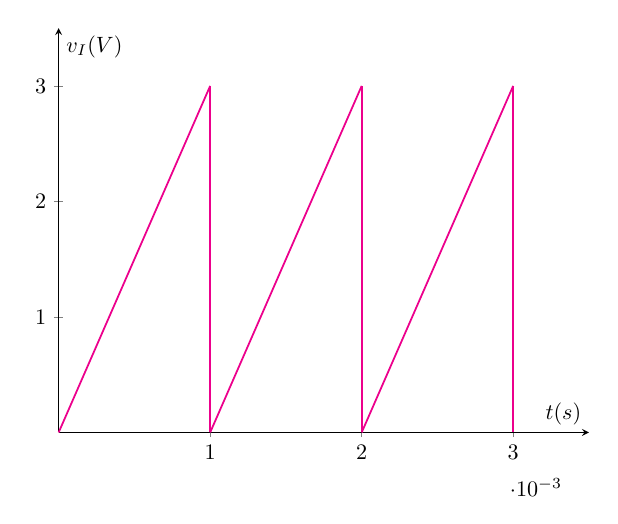
\begin{tikzpicture}[scale=0.8, transform shape]
		\pgfplotsset{width=10cm,height=8cm,compat=1.18}
		\begin{axis}[xshift=6cm,
			yshift=2cm,
			clip=false,
			axis y line=left,
			axis x line=middle,
			%grid style={line width=.1pt, draw=gray!20},
			%grid=both,
			%minor tick num=1,
			xlabel=$\quad t (s)$,
			ylabel=$v_I (V)$, 
			axis y line= center,
			xmin=0,xmax=0.0035,
			ymin=0,ymax=3.5,
			xtick={0, 0.001, 0.002, 0.003},
			ytick={0,1,2,3},
			%xticklabels={$$},
			%yticklabels={$V_{CC}$},
			]
			\addplot[smooth, magenta,thick, mark=none, domain=0:0.001, samples=200] {3000*x};
			\addplot[smooth, magenta,thick, mark=none, domain=0.001:0.002, samples=200] {3000*(x - 0.001)};
			\addplot[smooth, magenta,thick, mark=none, domain=0.002:0.003, samples=200] {3000*(x - 0.002)};
			\addplot[color = magenta, thick] coordinates {(0.001,3) (0.001,0)}; %vertical1
			\addplot[color = magenta, thick] coordinates {(0.002,3) (0.002,0)}; %vertical2
			\addplot[color = magenta, thick] coordinates {(0.003,3) (0.003,0)}; %vertical3
		\end{axis}
	\end{tikzpicture}
	\caption{Señal de entrada}	
	\label{fig:figura13}
\end{figure}

Se diseña una red divisora de tensión para atenuar la señal de entrada a un valor de $\qty{75}{\milli \volt}$ 

\begin{figure}[H]
	\centering	
	\begin{tikzpicture}[scale=0.8]
		\ctikzset{bipoles/thickness=4}
		\ctikzset{monopoles/vcc/arrow={Stealth[width=6pt,length=9pt]}}
		\ctikzset{monopoles/vee/arrow={Stealth[width=6pt,length=9pt]}}
		\draw (0,0) node[vcc](VCC){$+V_{CC}$} to[R, l=$R_c$] ++(0,-3) coordinate (p1)
		to[short, -o] ++(2,0) node[right]{$V_b = \qty{75}{\milli \volt}$};
		\draw (p1) to[R, *-, l=$R_d$] ++(0,-3) node[ground]{};
	\end{tikzpicture}
	\caption{Red divisora de voltaje }	
	\label{fig:figura14}
\end{figure}

Establecemos una corriente de $\qty{15}{\micro \ampere}$ y determinamos $R_d$
\begin{align}
	R_d = \frac{\qty{75}{\milli \volt}}{\qty{15}{\micro \ampere}} = \qty{5}{\kilo \ohm}
\end{align}

Ahora, determinamos el valor de $R_c$

\begin{align}
	R_c = \frac{\qty{15}{\volt} - \qty{75}{\milli \volt} }{\qty{3}{\micro \ampere}} = \qty{195}{\kilo \ohm}
\end{align}

\begin{figure}[H]
	\centering
	\begin{tikzpicture}[scale=0.8]
		\ctikzset{bipoles/thickness=4}
		\ctikzset{monopoles/vcc/arrow={Stealth[width=6pt,length=9pt]}}
		\ctikzset{monopoles/vee/arrow={Stealth[width=6pt,length=9pt]}}
		\draw (0,0) node[op amp](OA){};
		\draw (OA.-) to[short] ++(-1,0) to[short] ++(0,2) coordinate(p1);
		\draw (p1) to[short] (p1 -| OA.out) to[short] (OA.out);
		\draw (OA.+) to[short, -o] ++(-2,0) node[left]{$V_s$};
		\draw (OA.out) to[short, *-] ++(1,0) coordinate (p2)
		      to[R, l=$R_c$, a=$\qty{195}{\kilo \ohm}$] ++(0,-3) coordinate (p3)
		      to[R, l=$R_d$, a=$\qty{5}{\kilo \ohm}$] ++(0,-3) node[ground]{};
		\draw (p3) to[short, *-] ++(3,0) coordinate(p4);
		\draw (p4) node[op amp, anchor=+](OA1){};
		\draw (OA1.-) to[short] ++(-1,0) to[short] ++(0,2) coordinate (p5);
		\draw (p5) to[short] (p5 -| OA1.out) to[short] (OA1.out) to[short, *-o] ++(1,0) node[right]{$V_{o_1}$};
	\end{tikzpicture}
	\caption{Etapa acondicionadora para la señal de entrada}	
	\label{fig:figura15}
\end{figure}

\begin{figure}[H]
	\centering
	\scalebox{.8}{
		\begin{tikzpicture}[scale=0.8]
			\ctikzset{bipoles/thickness=4}
			\ctikzset{monopoles/vcc/arrow={Stealth[width=6pt,length=9pt]}}
			\ctikzset{monopoles/vee/arrow={Stealth[width=6pt,length=9pt]}}
			\draw (0,0) node[op amp, anchor=+](OA1){$OA_1$};
			\draw (OA1.-) to[short] ++(-1,0)
			to[short] ++(0,2) coordinate (p2);
			\draw (p2) to[short] (p2 -| OA1.out)
			to[short, -*] (OA1.out)
			to [R, l=$R_4$, a=$\qty{10}{\kilo \ohm}$] ++(3,0) coordinate (o1);
			\draw (OA1.+) to[short] ++(-2.5,0) coordinate (z1);
			\draw (z1) to[R, l=$R_d$] ++(0,-3) node[ground]{};
			\draw (z1) to[R, l_=$R_c$, *-] ++(0,3) to[short] ++(-1,0) coordinate (z2);
			\draw (z2) node[op amp, anchor=out](OA5){$OA_5$};
			\draw (OA5.-) to[short] ++(-1,0) to[short] ++(0,2) coordinate(z3);
			\draw (z3) to[short] (z3 -| OA5.out) to[short, -*] (OA5.out);
			\draw (OA5.+) to[short, -o] ++(-1,0) node[left]{$V_s$};
			\draw (o1) to[short] ++(0, 2) coordinate (p3);
			\draw (o1) to[short, *-] ++(1,0) node[op amp, anchor=-](OA2){$OA_2$};
			\draw (p3) to[R, l=$R_3$, a=$\qty{10}{\kilo \ohm}$] (p3 -| OA2.out)
			to[short] (OA2.out);
			\draw (OA2.out) to[R, *-, l=$R_1$, a=$\qty{750}{\ohm}$] ++(4,0) coordinate (p5)
			to[short] ++(0,-5)
			to[R, l_=$R_2$, a^=$\qty{20}{\kilo \ohm}$] ++(-4,0) coordinate (o2);
			\draw (o2) node[op amp, anchor=out](OA3){$OA_3$};
			\draw (OA3.-) to[short] ++(-1,0)
			to[short] ++(0,2) coordinate (p6);
			\draw (p6) to[short] (p6 -| OA3.out) to[short, -*] (OA3.out);
			\draw (OA3.+) to[short] ++(-3,0) coordinate (p7);
			\draw (p7) to[R, *-, l_=$R_a$, a^=$\qty{1.4}{\mega \ohm}$] ++(0,3) node[vcc](VCC){$+V_{CC}$};
			\draw (p7) to[R, l=$R_b$, a=$\qty{100}{\kilo \ohm}$] ++(0,-3) node[ground]{};
			\draw (OA2.+) to[short] ++(-1,0) node[ground]{};
			\draw (p5) to[short, *-] ++(0.5,0) coordinate(p8);
			\draw (p8) to[short] ++(1,0) node[op amp, anchor=-](OA4){$OA_4$};
			\draw (p8) to[short, *-] ++(0,2.5) coordinate (p10);
			\draw (p10) to[R, l=$R_F$, a=$\qty{100}{\kilo \ohm}$] (p10 -| OA4.out) to[short, -*] (OA4.out)
			to[short, -o] ++(1,0) node[right]{$v_o$};
			\draw (OA4.+) to[short] ++(-0.5,0) node[ground]{};
			\draw(OA4.up) to[short] ++(0,0.4) node[vcc](VCC){$+V_{CC}$};
			\draw(OA4.down) to[short] ++(0,-0.4) node[vee](VEE){$-V_{EE}$};
	\end{tikzpicture}}
	\caption{Circuito completo}	
	\label{fig:figura16}
\end{figure}

\begin{figure}[H]
	\centering
	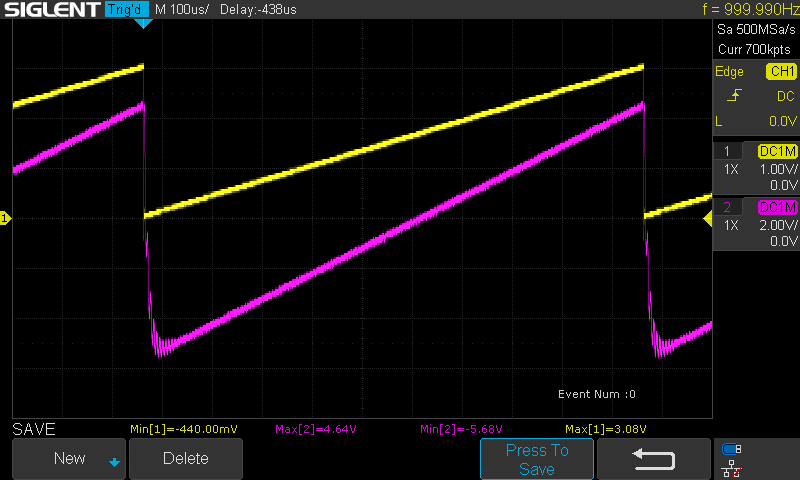
\includegraphics[width=\textwidth]{SDS00033}
	\caption{Voltaje de salida (morado) y voltaje de entrada original (amarillo)}	
	\label{fig:figura4}
\end{figure}


\begin{figure}[H]
	\centering
	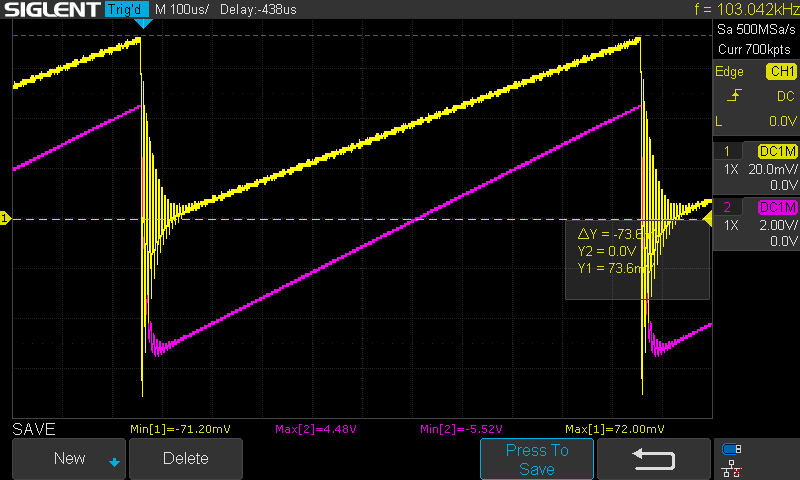
\includegraphics[width=\textwidth]{SDS00031}
	\caption{Voltaje de salida (morado) y voltaje de entrada escalado (amarillo)}	
	\label{fig:figura17}
\end{figure}

\begin{figure}[H]
	\centering
	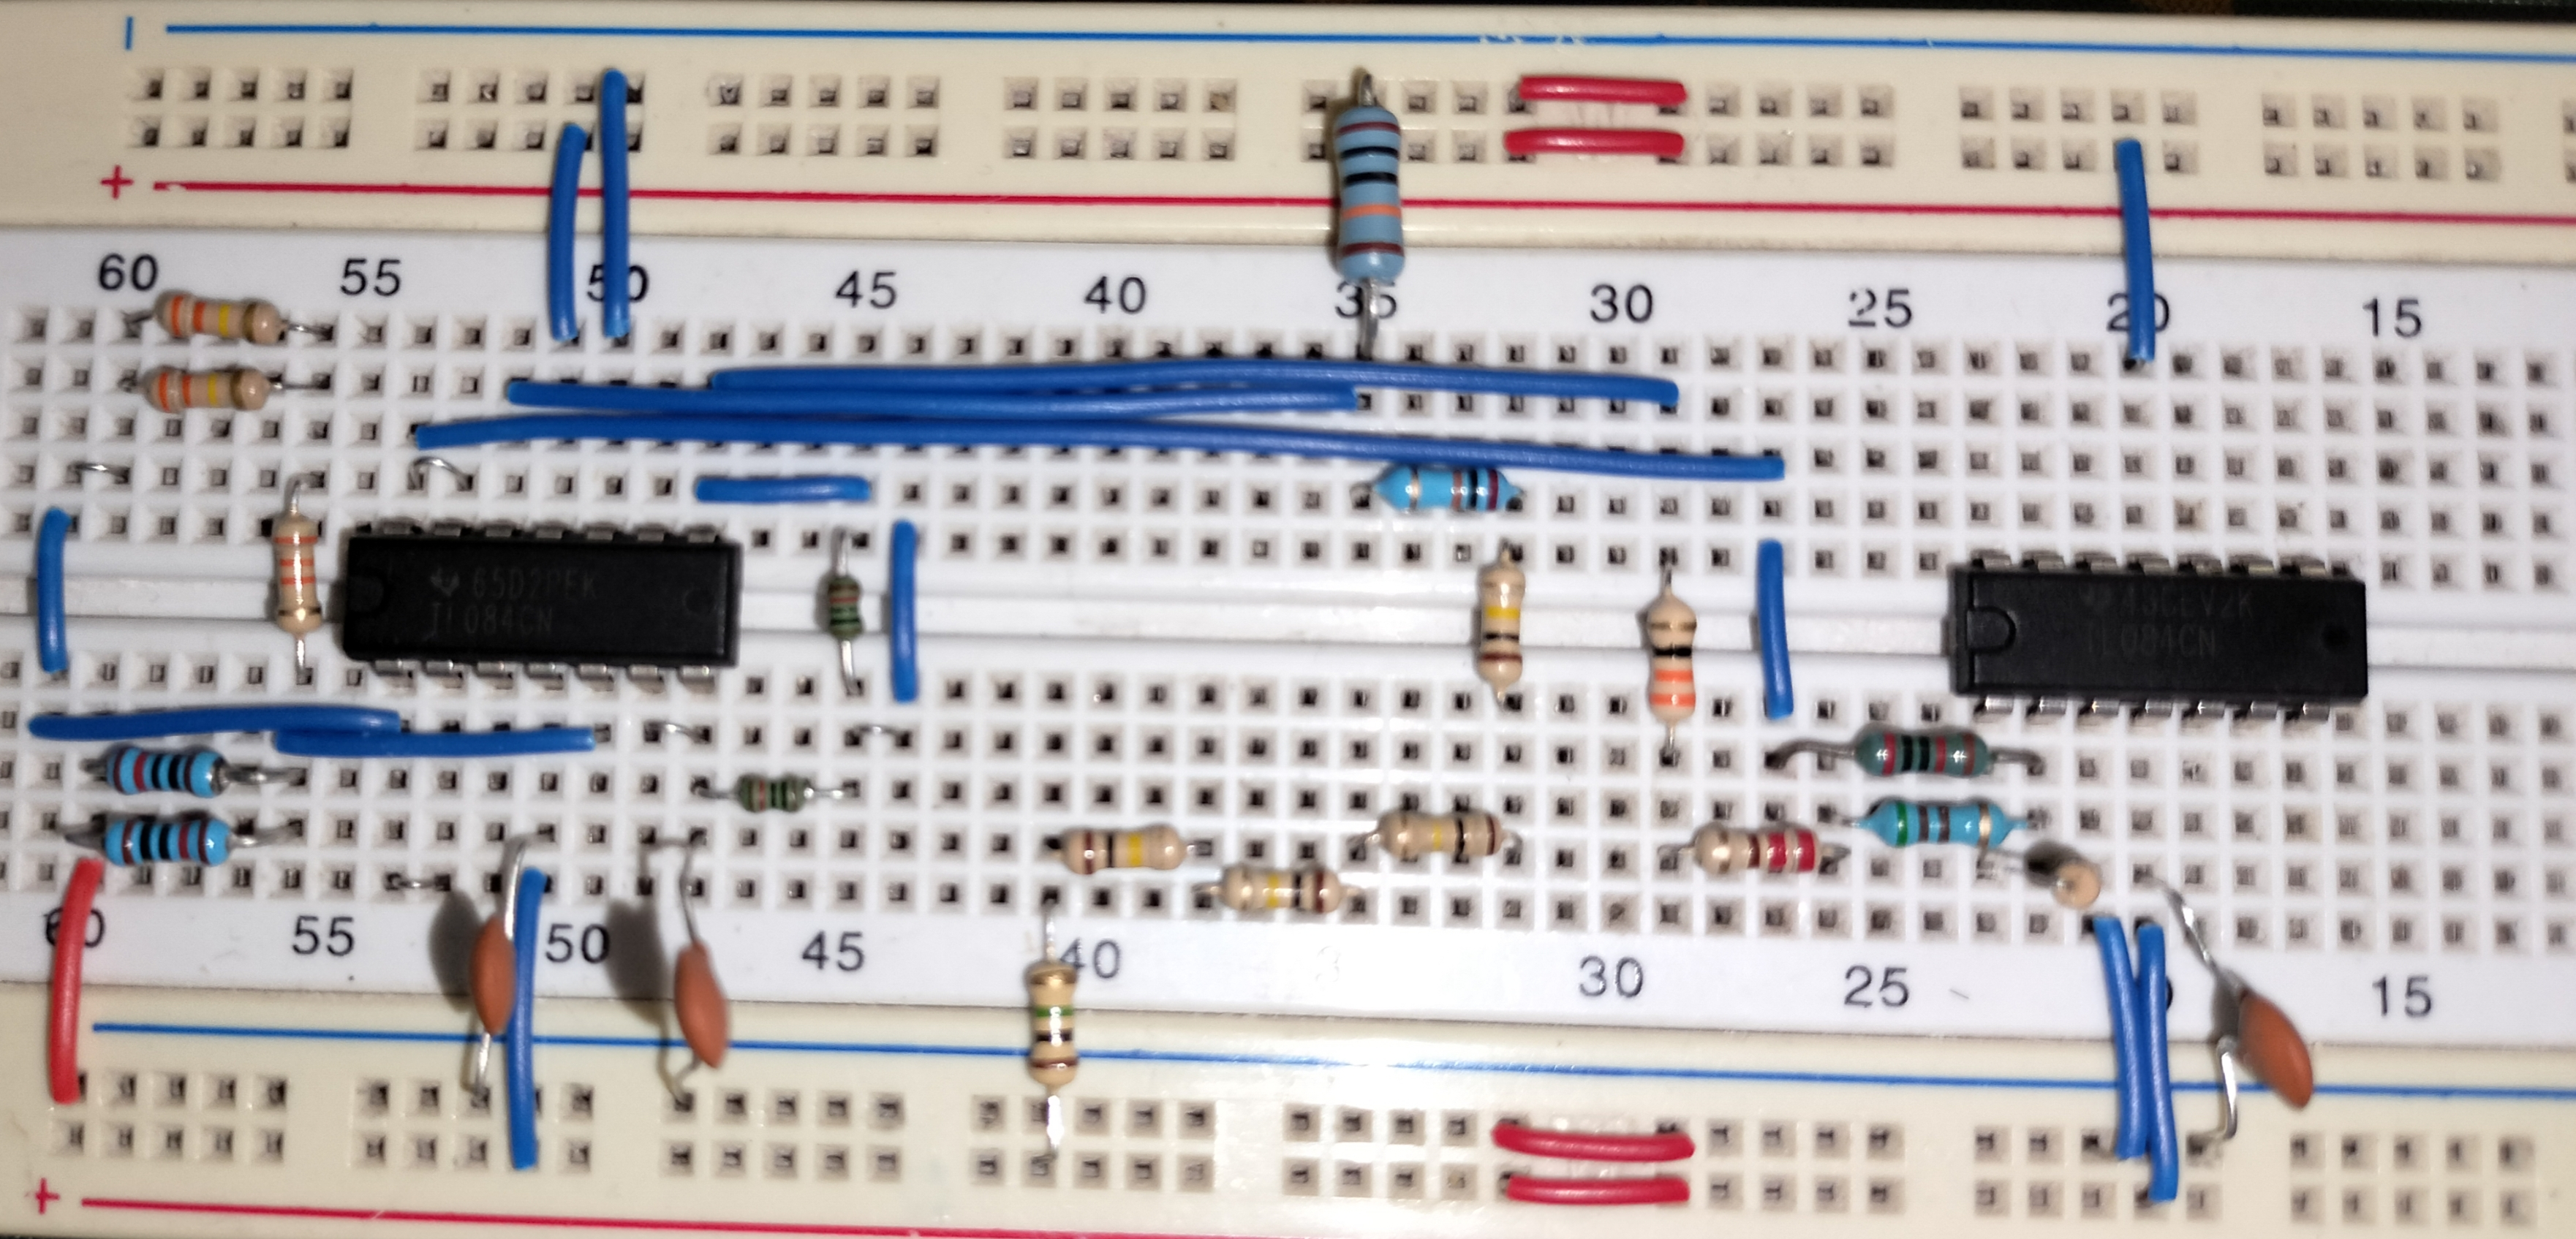
\includegraphics[width=\textwidth]{proto}
	\caption{Voltaje de salida (morado) y voltaje de entrada escalado (amarillo)}	
	\label{fig:figura18}
\end{figure}



\end{document}